\tightsection{Quality Improvement via Prediction}
Now we can fill in the details of section 3 a bit more.  Figure~\ref{fig:go-overview} shows how prediction and decision-making work in GO.
\begin{figure}[h!]
\centering
 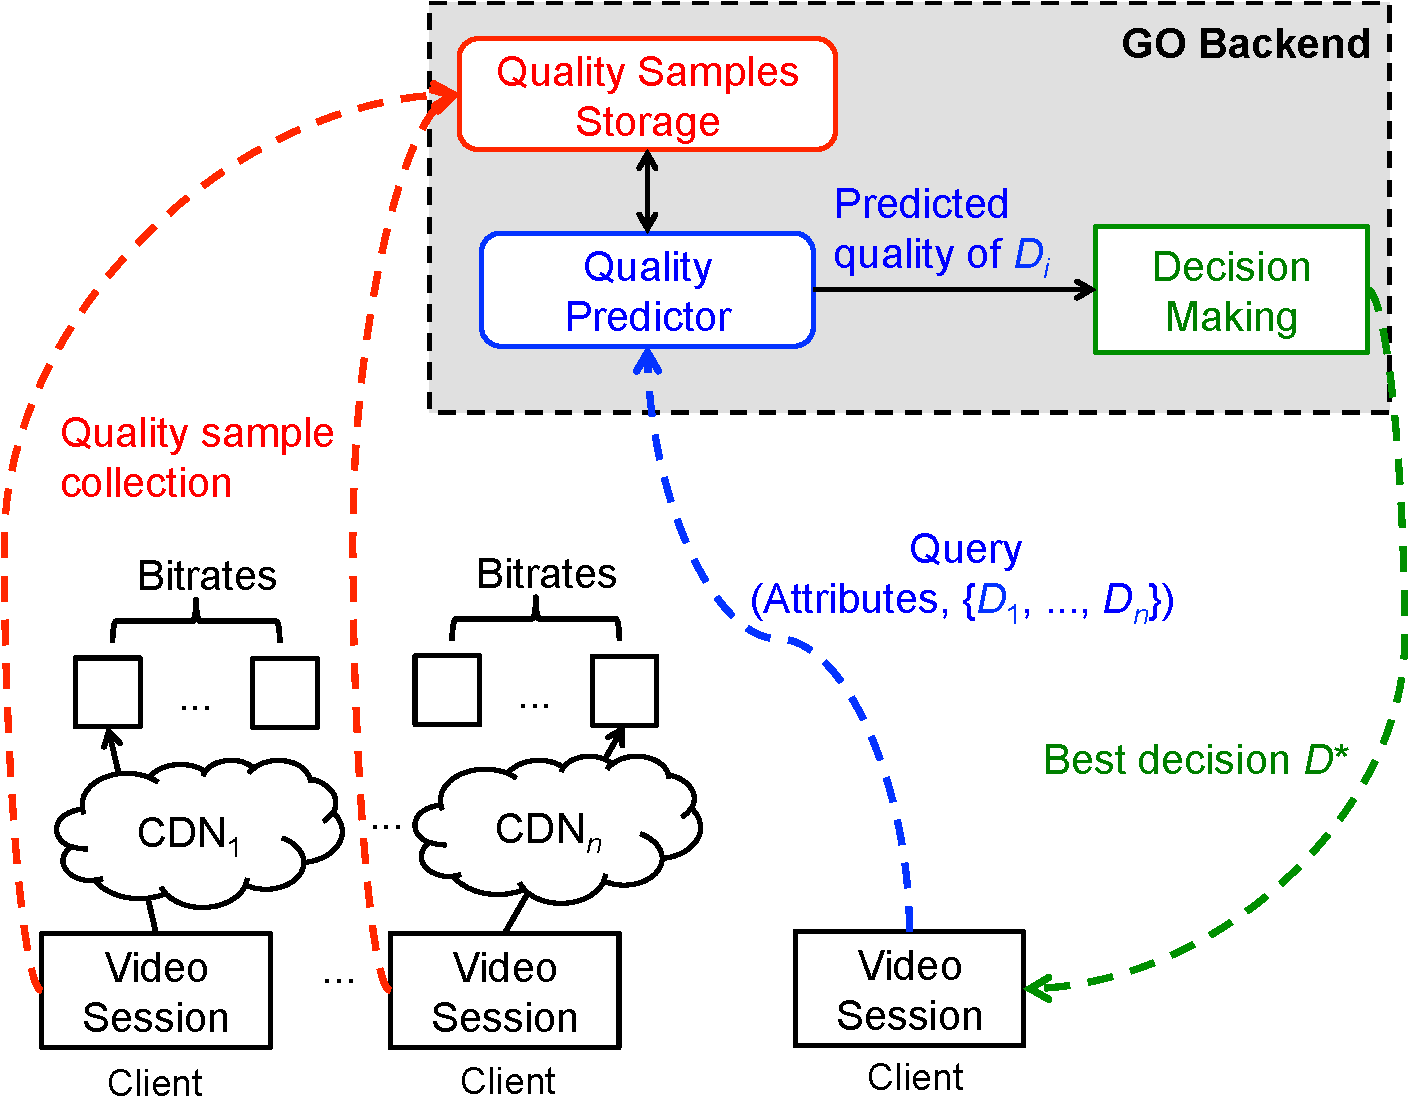
\includegraphics[width=0.5\textwidth] {figures/go-overview.pdf}
\tightcaption{Architecture of GO.}
\label{fig:go-overview}
\end{figure}

\tightsubsection{Behavioral study}
To build confidence in this algorithm, we show you how decision-making based on prediction behaves in some simple synthetic scenarios where the optimal decisions are clear:
\begin{packedenumerate}
  \item A sudden change in CDN performance causes relative performance to change.
  \item One CDN performs better for one group (under an observed attribute) and worse for another group.
\end{packedenumerate}

\tightsubsection{Evaluation against a baseline}
We show how this works in practice in a real trace, in comparison to random decisions.

\tightsubsection{Evaluation against an oracle}
In real traces, it is impractical to identify an optimal alternative.  Instead, we generate a synthetic dataset which models some of the complexities of the real-world dataset but which admits an oracle.  We analyze the performance of GO in comparison to the oracle.  Separately from the GO algorithm, it is also interesting to see how prediction error impacts quality outcomes in this synthetic scenario.  We add random noise to the oracle’s predictions (reflecting an admittedly simplistic model of prediction error) and show how larger amounts of noise impact quality outcomes.  This also allows us to say that GO’s performance is equivalent to that of an oracle with a certain amount of random noise.
